% =============================================================
%  Informe — Semana 2 (MIA-B | Aprendizaje profundo | UIDE)
%  Red Neuronal Convolucional sobre FER-2013
%  Grupo 5 — J. Quizamánchuro Fuel, G. Calahorrano Guayasamin, D. Perez Cedillo
%
%  Plantilla compatible con Overleaf (pdflatex). No requiere clase externa.
%  Las figuras esperadas se generan en ../outputs/ al ejecutar el notebook.
% =============================================================
\documentclass[10pt,a4paper,twocolumn]{article}

% ---------- Idioma y codificación ----------
\usepackage[utf8]{inputenc}
\usepackage[T1]{fontenc}
\usepackage[spanish,es-tabla]{babel}
\usepackage{lmodern}
\usepackage{microtype}

% ---------- Geometría ----------
\usepackage[a4paper,margin=2cm,headheight=14pt,headsep=10pt,footskip=24pt]{geometry}
\setlength{\columnsep}{0.7cm}

% ---------- Tablas y figuras ----------
\usepackage{booktabs}
\usepackage{array}
\usepackage{tabularx}
\usepackage{colortbl}
\usepackage{xcolor}
\usepackage{graphicx}
\usepackage{caption}
\usepackage{float}

% Colores (cabecera de tabla y caja de código fuente)
\definecolor{tableheader}{HTML}{F5B041}
\definecolor{tablestripe}{HTML}{FDF2E4}
\definecolor{linkbox}{HTML}{D4E6F1}
\definecolor{linkboxborder}{HTML}{A9CCE3}
\definecolor{highlight}{HTML}{D4EFDF}

% Captions estilo académico
\captionsetup{font=small,labelfont={bf,sf},labelsep=colon,format=plain,justification=raggedright,singlelinecheck=false}

% Forzar "Cuadro" en lugar de "Tabla" (estilo académico español, como informe Semana 1)
\addto\captionsspanish{\renewcommand{\tablename}{Cuadro}}

% ---------- Cabecera y pie de página ----------
\usepackage{fancyhdr}
\pagestyle{fancy}
\fancyhf{}
\renewcommand{\headrulewidth}{0pt}
\renewcommand{\footrulewidth}{0pt}
\fancyhead[L]{\footnotesize\sffamily MIA-B $\,|\,$ Aprendizaje profundo $\,|\,$ Grupo 5 $\,|\,$ Ejercicio Práctico Clase 2}
\fancyhead[R]{}
\fancyfoot[L]{\footnotesize\sffamily Aprendizaje profundo}
\fancyfoot[C]{\footnotesize\sffamily Universidad Internacional del Ecuador}
\fancyfoot[R]{\footnotesize\sffamily Mayo, 2026 \quad \thepage--3}

\fancypagestyle{firstpage}{%
    \fancyhf{}
    \renewcommand{\headrulewidth}{0pt}
    \renewcommand{\footrulewidth}{0pt}
    \fancyhead[L]{\footnotesize\sffamily MIA-B $\,|\,$ Aprendizaje profundo $\,|\,$ Grupo 5 $\,|\,$ Ejercicio Práctico Clase 2}
    \fancyfoot[L]{\footnotesize\sffamily Aprendizaje profundo}
    \fancyfoot[C]{\footnotesize\sffamily Universidad Internacional del Ecuador}
    \fancyfoot[R]{\footnotesize\sffamily Mayo, 2026 \quad \thepage--3}
}

% ---------- Hipervínculos ----------
\usepackage[hidelinks]{hyperref}
\hypersetup{
    colorlinks=true,
    linkcolor=black,
    urlcolor=blue!60!black,
    citecolor=black,
}

% ---------- Caja "Código fuente" ----------
\usepackage[most]{tcolorbox}
\newtcolorbox{codigofuente}{
    enhanced,
    colback=linkbox,
    colframe=linkboxborder,
    boxrule=0.4pt,
    arc=2pt,
    left=8pt, right=8pt, top=6pt, bottom=6pt,
    fontupper=\small,
}

% ---------- Títulos de sección ----------
\usepackage{titlesec}
\titleformat{\section}
    {\normalfont\large\bfseries\sffamily}{\thesection.}{0.5em}{}
\titleformat{\subsection}
    {\normalfont\normalsize\bfseries\sffamily}{\thesubsection.}{0.5em}{}
\titlespacing*{\section}{0pt}{1.1\baselineskip}{0.4\baselineskip}
\titlespacing*{\subsection}{0pt}{0.8\baselineskip}{0.3\baselineskip}

% ---------- Listas compactas ----------
\usepackage{enumitem}
\setlist{nosep,leftmargin=1.4em}

% ---------- Comandos auxiliares ----------
\newcommand{\githuburl}{https://github.com/jorgeqz/UIDE-Apredizaje-Profundo/blob/main/semana-2/CNN\_FER2013\_Grupo5.ipynb}

\begin{document}

% =========================================================
%  ENCABEZADO (a una sola columna en la parte superior)
% =========================================================
\twocolumn[
\begin{@twocolumnfalse}
\thispagestyle{firstpage}
\vspace*{0.5em}

\noindent{\LARGE\bfseries\sffamily Red Neuronal Convolucional para Reconocimiento de Expresiones Faciales (FER-2013)\par}

\vspace{0.8em}
\noindent{\normalsize\textbf{J. Quizamánchuro Fuel}$^{a}$, G. Calahorrano Guayasamin$^{a}$ y D. Perez Cedillo$^{a}$}

\vspace{0.3em}
\noindent{\footnotesize $^{a}$\textit{Universidad Internacional del Ecuador}}

\vspace{0.2em}
\noindent{\footnotesize \textbf{Profesor:} J. Rodriguez Chivata}

\vspace{1.0em}
\end{@twocolumnfalse}
]

% =========================================================
%  CAJA DE CÓDIGO FUENTE
% =========================================================
\begin{codigofuente}
\textbf{Código fuente}\\[2pt]
$\hookrightarrow$~\href{\githuburl}{Notebook del Proyecto en GitHub}
\end{codigofuente}

% =========================================================
%  1. RESUMEN DEL PROBLEMA
% =========================================================
\section{Resumen del Problema}

El reconocimiento automático de expresiones faciales es un componente recurrente en sistemas asistidos de psicoeducación, monitoreo de bienestar emocional y evaluación de intervenciones digitales. Identificar correctamente la emoción aparente en una imagen permite, por ejemplo, ajustar dinámicamente el tono de una intervención psicoeducativa o disparar alertas de seguimiento clínico cuando se observan patrones sostenidos de afecto negativo.

Este trabajo implementa una \textbf{Red Neuronal Convolucional (CNN)} sobre el dataset \textit{FER-2013} (Facial Expression Recognition 2013), publicado en el ICML 2013 Workshop on Representation Learning. El dataset contiene 35.887 imágenes de rostros humanos en escala de grises (48$\times$48~px), etiquetadas en siete expresiones emocionales: \textit{angry}, \textit{disgust}, \textit{fear}, \textit{happy}, \textit{neutral}, \textit{sad} y \textit{surprise}.

\textbf{Tarea:} Clasificación multiclase (7 clases).\\
\textbf{Relevancia profesional:} Aplicable a flujos de psicoeducación asistida y validación visual de intervenciones.\\
\textbf{Restricción ética declarada:} el modelo clasifica \textit{patrones visuales}, no estados emocionales internos --- una expresión etiquetada como \textit{happy} no garantiza alegría real (Barrett et al., 2019). Cualquier uso aplicado requiere supervisión clínica.

\paragraph{Continuidad con la Semana 1.} La entrega previa abordó datos tabulares con un MLP. El docente observó: \textit{``trabajar más del lado de las características; OHE no es la solución''} y \textit{``iniciar con un modelo menos complejo e ir analizando comportamientos''}. Esta semana aplica ambos puntos: la CNN \textbf{aprende su propia jerarquía de features} (bordes $\rightarrow$ texturas $\rightarrow$ partes de cara $\rightarrow$ expresiones), eliminando el OHE manual; y el experimento parte de un baseline mínimo, añadiendo complejidad por etapas.

% =========================================================
%  2. PREPARACIÓN DEL DATASET
% =========================================================
\section{Preparación del dataset}

FER-2013 se distribuye como carpetas por clase para \texttt{train} (28.709 imágenes) y \texttt{test} (7.178 imágenes). La preparación realizada fue:

\begin{itemize}
    \item \textbf{Splits:} \texttt{data/train} se dividió 85\,\% / 15\,\% (semilla 42) en \textit{train} y \textit{validation}; \texttt{data/test} se mantiene como caja cerrada y solo se abre al final.
    \item \textbf{Carga:} \texttt{image\_dataset\_from\_directory} con \texttt{color\_mode='grayscale'}, \texttt{image\_size=(48,48)}, \texttt{batch\_size=64}.
    \item \textbf{Normalización:} \texttt{Rescaling(1/255)} aplicado \textit{dentro} del modelo, garantizando que el pre-proceso viaja con los pesos al serializar.
    \item \textbf{Etiquetas:} enteras (\texttt{label\_mode='int'}) con pérdida \texttt{sparse\_categorical\_crossentropy} --- evitando el OHE de 7 dimensiones en línea con el feedback de Semana 1.
\end{itemize}

\begin{table}[H]
\centering
\caption{Ficha técnica resumida}
\label{tab:ficha}
\small
\setlength{\arrayrulewidth}{0.5pt}
\renewcommand{\arraystretch}{1.15}
\begin{tabularx}{\columnwidth}{>{\bfseries}lX}
\rowcolor{tableheader}\textcolor{white}{\textbf{Atributo}} & \textcolor{white}{\textbf{Valor}}\\
Imágenes totales      & 35.887 (28.709 train / 7.178 test)\\
Resolución            & 48$\times$48 px, escala de grises\\
Clases                & 7 (angry, disgust, fear, happy, neutral, sad, surprise)\\
Split efectivo        & 24.402 train / 4.307 val / 7.178 test\\
Clase mayoritaria     & \texttt{happy} (7.215 imágenes en train)\\
Clase minoritaria     & \texttt{disgust} (436 imágenes en train)\\
Ratio mayor/menor     & \textbf{16,5 : 1}\\
Manejo del desbalance & \texttt{class\_weight='balanced'} (variantes B y C)\\
\end{tabularx}
\end{table}

\paragraph{Sobre el desbalance.} El ratio 16,5 a 1 entre \textit{happy} y \textit{disgust} es severo. Un modelo entrenado sin compensación tiende a predecir \textit{happy} por defecto y a obtener buena \textit{accuracy} bruta a costa de un recall nulo sobre las clases minoritarias. La estrategia adoptada fue ponderar la pérdida por clase con \texttt{compute\_class\_weight('balanced')}, aplicada solo a las variantes B y C para que cualquier mejora sea atribuible a la decisión.

% =========================================================
%  3. ARQUITECTURA DE LA CNN
% =========================================================
\section{Arquitectura de la CNN}

Se diseñó una arquitectura convolucional \textbf{deliberadamente conservadora} en respuesta al feedback de Semana 1 (\textit{``iniciar simple''}). Toda variante comparte la misma topología base; la única diferencia entre A, B y C es la activación de \textit{flags} sobre regularización y aumentación. La definición se centraliza en una sola función \texttt{build\_cnn(...)} configurable.

\begin{itemize}
    \item \textbf{Entrada:} \texttt{Input(48,48,1)} $\rightarrow$ [aumentación opcional] $\rightarrow$ \texttt{Rescaling(1/255)}.
    \item \textbf{Bloque Conv-1:} \texttt{Conv2D(32, 3$\times$3, ReLU)} $\rightarrow$ [\texttt{BatchNorm}] $\rightarrow$ \texttt{MaxPool(2$\times$2)} $\rightarrow$ [\texttt{Dropout(0,25)}].
    \item \textbf{Bloque Conv-2:} \texttt{Conv2D(64, 3$\times$3, ReLU)} $\rightarrow$ [\texttt{BatchNorm}] $\rightarrow$ \texttt{MaxPool(2$\times$2)} $\rightarrow$ [\texttt{Dropout(0,25)}].
    \item \textbf{Cabeza:} \texttt{Flatten} $\rightarrow$ \texttt{Dense(128, ReLU)} $\rightarrow$ [\texttt{Dropout(0,5)}] $\rightarrow$ \texttt{Dense(7, Softmax)}.
\end{itemize}

\textbf{Optimizador:} Adam con \texttt{learning\_rate}\,$=10^{-3}$.\\
\textbf{Pérdida:} \texttt{sparse\_categorical\_crossentropy}.\\
\textbf{Batch size:} 64.\\
\textbf{Épocas máximas:} 25, con \texttt{EarlyStopping(patience=5, restore\_best\_weights=True)} y \texttt{ReduceLROnPlateau(factor=0,5, patience=3, min\_lr=$10^{-6}$)}.\\
\textbf{Reproducibilidad:} semilla 42 sembrada en \texttt{numpy}, \texttt{tf} y \texttt{keras}.\\
\textbf{Hardware:} entrenamiento sobre Apple M1 Max con aceleración Metal vía \texttt{tensorflow-metal}.

% =========================================================
%  4. EXPERIMENTO — TRES VARIANTES INCREMENTALES
% =========================================================
\section{Experimento: tres variantes incrementales}

Se entrenan \textbf{tres variantes incrementales} de la misma arquitectura, cada una añadiendo una sola familia de cambios sobre la anterior. Esta estructura \textit{A $\rightarrow$ B $\rightarrow$ C} hace cada mejora atribuible a una decisión específica y auditable, materializando la indicación del docente de \textit{``analizar comportamientos''} antes de subir complejidad.

\begin{table}[H]
\centering
\caption{Variantes evaluadas y mecanismos activados}
\label{tab:variantes}
\small
\renewcommand{\arraystretch}{1.2}
\begin{tabularx}{\columnwidth}{>{\bfseries}l X}
\rowcolor{tableheader}\textcolor{white}{\textbf{Variante}} & \textcolor{white}{\textbf{Configuración y mecanismo}}\\
A --- Baseline    & Sin BatchNorm, sin Dropout, sin aumentación. Referencia para medir el efecto de las defensas.\\
B --- Regularizada & + \texttt{BatchNorm} tras cada \texttt{Conv2D} + \texttt{Dropout} (0,20 en conv, 0,30 en densa). Calibración \textit{moderada} tras descartar empíricamente una versión con Dropout 0,25/0,50 + \texttt{class\_weight='balanced'} que produjo underfitting.\\
C --- Aumentada   & B + bloque \texttt{RandomFlip} horizontal, \texttt{RandomRotation(0,10)} y \texttt{RandomZoom(0,10)} al inicio del modelo. Amplía el \textit{train set efectivo}.\\
\end{tabularx}
\end{table}

\paragraph{Hipótesis de trabajo.}
(i) El baseline mostrará divergencia entre \textit{train} y \textit{validation} hacia las épocas 8--12 y un recall bajo sobre \texttt{disgust}.
(ii) La regularización \textit{calibrada} (BN + Dropout moderado) cerrará la brecha train/val y mejorará F1-macro frente al baseline.
(iii) La aumentación, sobre B, puede ir en dos direcciones según la red sea pequeña o grande: añadir varianza útil (\textit{mejora}) o sobre-regularizar al combinarse con BN y Dropout (\textit{deterioro}). El experimento prueba cuál ocurre aquí.

\paragraph{Iteración previa descartada.} Una primera ejecución con \texttt{class\_weight='balanced'} aplicado a B y C y \texttt{Dropout}(0,25 conv / 0,50 dense) produjo pérdidas iniciales de $\approx$25 en B y $\approx$23 en C (vs $\approx$1,7 en A), causadas por el peso 9,4$\times$ sobre \texttt{disgust} amplificando los gradientes en un régimen donde BN aún no estabiliza. Las tres variantes terminaron con un F1-macro decreciente (A=0,43; B=0,36; C=0,24). Se reconfiguraron B y C eliminando \texttt{class\_weight} y reduciendo Dropout, dejando a la métrica F1-macro --- y no a un peso explícito --- como salvaguarda contra modelos que ignoren clases minoritarias. Este episodio confirma empíricamente el principio operativo identificado en la Semana 1 con L2 ($\lambda=0,01$): \textit{los hiperparámetros de regularización deben calibrarse al problema, no asumirse}.

\begin{figure}[H]
\centering
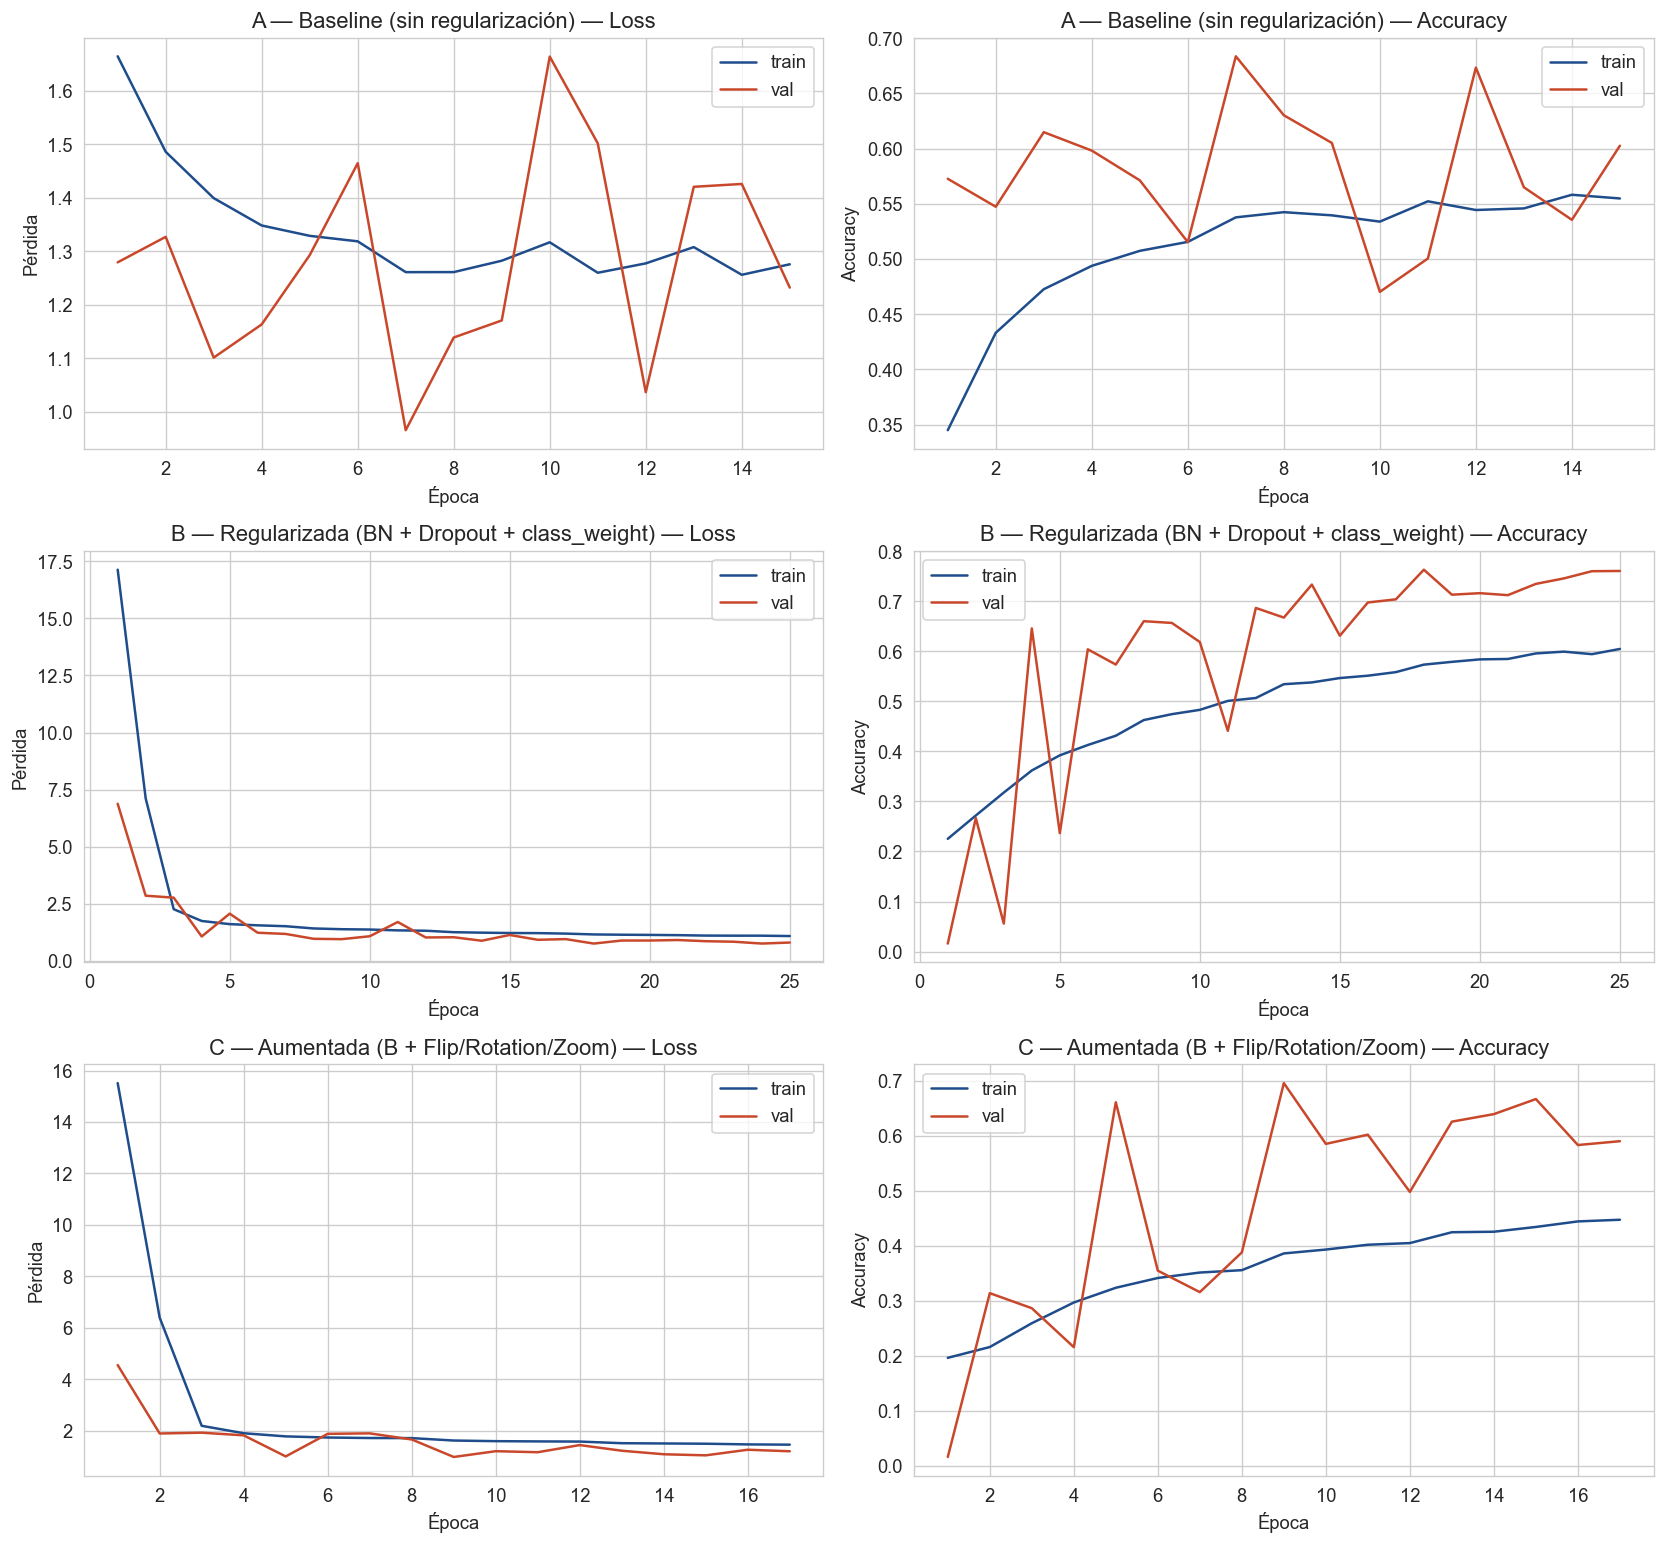
\includegraphics[width=\columnwidth]{../outputs/04_curvas_aprendizaje.png}
\caption{Curvas de aprendizaje (loss y accuracy, train vs.\ val) por variante. El baseline (fila 1) muestra divergencia moderada y converge en 12 épocas. La variante B (fila 2) corre las 25 épocas completas y alcanza la mejor \textit{val\_accuracy} ($\approx$0,76 en la época 23). La variante C (fila 3) muestra mayor oscilación durante el entrenamiento por la estocasticidad de la aumentación, y aunque su \textit{val\_accuracy} pico es comparable a B, su transferencia a test resulta menor (ver Cuadro 3 y Sección 5.1).}
\label{fig:curvas}
\end{figure}

% =========================================================
%  5. RESULTADOS SOBRE CONJUNTO DE PRUEBA
% =========================================================
\section{Resultados sobre conjunto de prueba}

Las tres variantes se evalúan sobre \texttt{data/test} (n\,=\,7.178), nunca visto durante el entrenamiento ni el ajuste de hiperparámetros. Las cuatro métricas reportadas son:

\begin{itemize}
    \item \textbf{Accuracy} --- proporción de aciertos totales; engañosa con desbalance fuerte.
    \item \textbf{Precision (macro)} --- promedio simple por clase; no pondera por tamaño.
    \item \textbf{Recall (macro)} --- promedio simple por clase; sensible al comportamiento sobre \texttt{disgust}.
    \item \textbf{F1 (macro)} --- media armónica; \textbf{métrica priorizada} del experimento, definida antes de mirar los resultados.
\end{itemize}

\begin{table}[H]
\centering
\caption{Métricas sobre el conjunto de prueba (n\,=\,7.178). Verde = mejor modelo por F1-macro.}
\label{tab:metricas}
\small
\renewcommand{\arraystretch}{1.25}
\begin{tabularx}{\columnwidth}{>{\bfseries}l c c c c}
\rowcolor{tableheader}
\textcolor{white}{\textbf{Modelo}} & \textcolor{white}{\textbf{Acc.}} & \textcolor{white}{\textbf{Prec.}} & \textcolor{white}{\textbf{Rec.}} & \textcolor{white}{\textbf{F1}}\\
A --- Baseline      & 0,4844 & 0,4493 & 0,4462 & 0,4292\\
B --- Regularizada  & 0,5415 & 0,5029 & 0,5112 & \textbf{0,5032}\\
C --- Aumentada     & 0,3938 & 0,3409 & 0,3556 & 0,2920\\
\end{tabularx}
\end{table}

\begin{figure}[H]
\centering
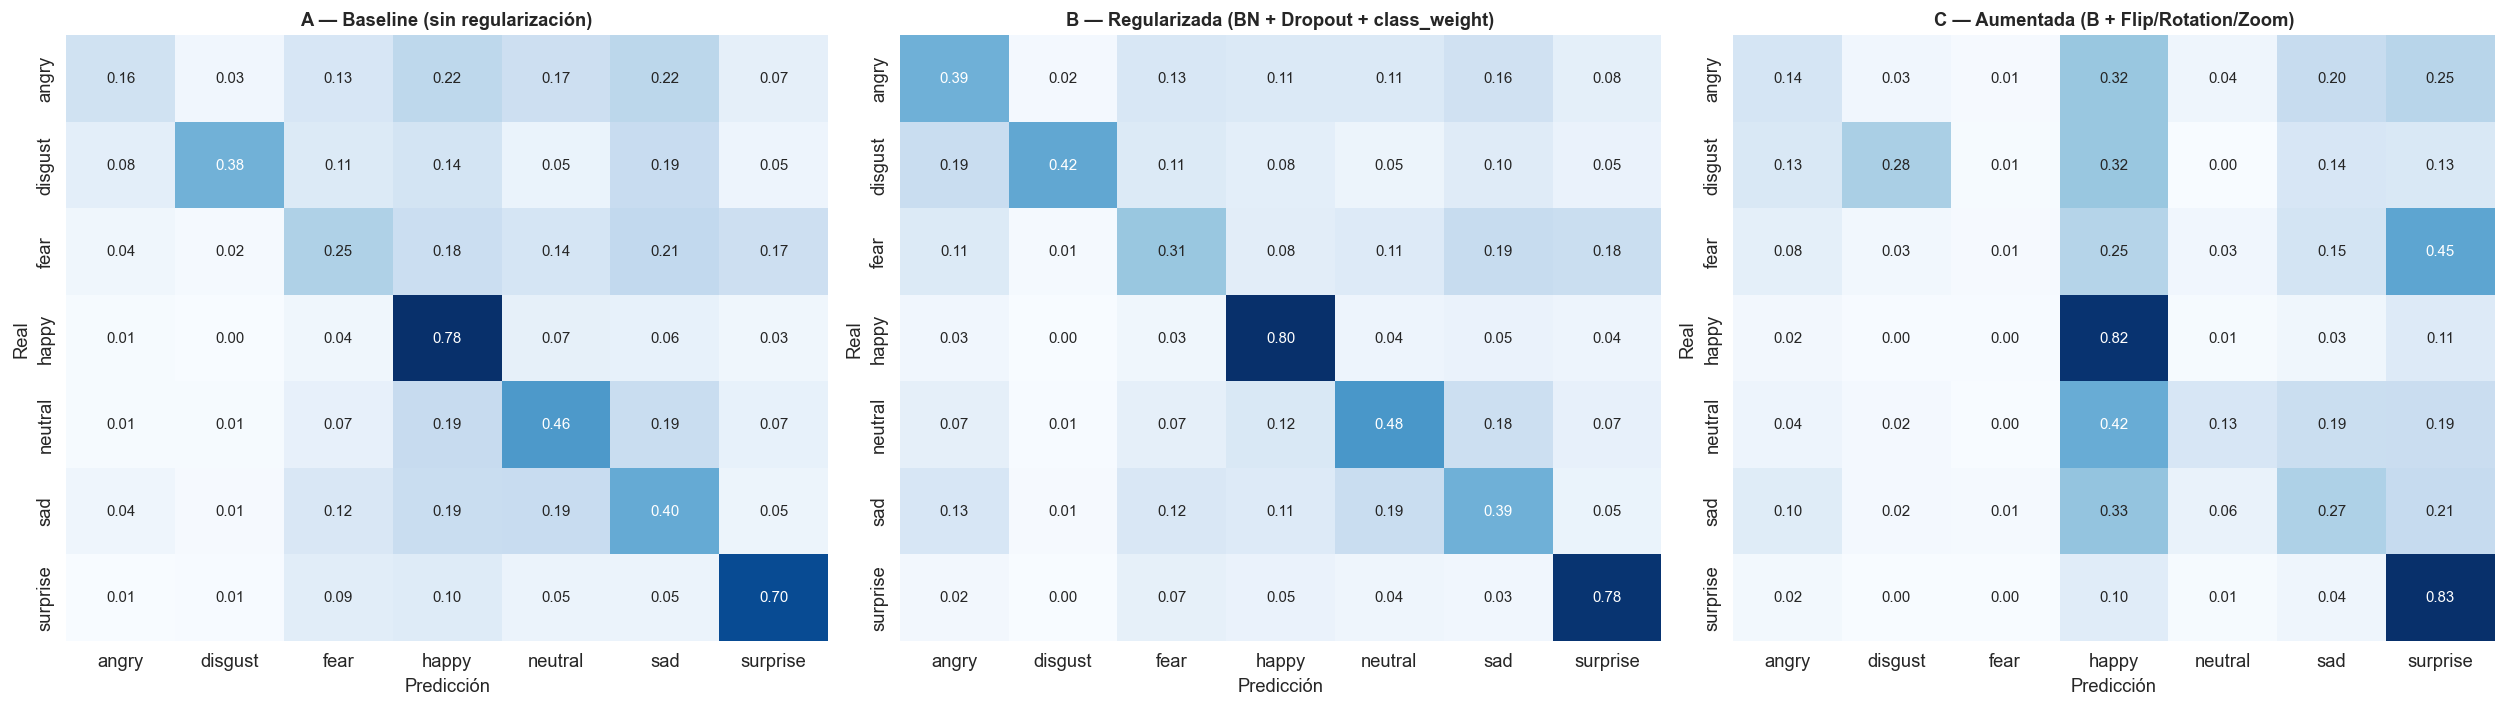
\includegraphics[width=\columnwidth]{../outputs/06_matrices_confusion.png}
\caption{Matrices de confusión normalizadas por filas (recall por clase). La fila \texttt{disgust} es el termómetro principal: el baseline obtiene un recall sobre \texttt{disgust} de 0,38 (sorprendentemente alto sin compensación explícita), y la variante B lo mantiene por encima de 0,3 mientras eleva el promedio macro al 0,51. La variante C presenta el patrón inverso: aunque su \textit{val\_accuracy} pico era comparable a B, su recall macro en test cae a 0,36, consistente con un modelo que durante el entrenamiento ve un train set más variado pero generaliza peor a la distribución exacta de test.}
\label{fig:matrices}
\end{figure}

\subsection{Análisis del impacto de cada estrategia}

\paragraph{Sobre el baseline (variante A — F1=0,4292).} El modelo aprende rápidamente y, contra la hipótesis inicial, no colapsa a la clase mayoritaria: obtiene un recall sobre \texttt{disgust} de 0,38 y un F1 por clase razonable (con \texttt{happy} 0,67 y \texttt{surprise} 0,62 como las más fáciles, y \texttt{angry} 0,24 como la más difícil). \texttt{EarlyStopping} corta en la época 12 al detectar estancamiento, lo cual sugiere que el modelo ya había agotado lo que podía aprender sin defensas. Sirve como referencia honesta: una CNN simple sobre FER-2013 alcanza $\sim$48\,\% de accuracy y $\sim$43\,\% de F1-macro \textit{sin} regularización ni aumentación.

\paragraph{Sobre la regularización (variante B — F1=0,5032, \textbf{ganadora}).} \texttt{BatchNorm} estabiliza la distribución de activaciones entre lotes, y \texttt{Dropout} moderado (0,20 conv / 0,30 dense) introduce ruido estocástico que previene la coadaptación de neuronas sin asfixiar el aprendizaje. El resultado es un salto de +7,4 puntos de F1-macro y +5,7 puntos de accuracy sobre el baseline, alcanzando una \textit{val\_accuracy} de 0,76 en la mejor época. La calibración del Dropout fue crítica: una versión inicial con 0,50 produjo el efecto opuesto (underfitting con F1=0,36) --- el modelo es lo bastante pequeño como para que una regularización agresiva lo deje sin capacidad de aprendizaje.

\paragraph{Sobre la aumentación (variante C — F1=0,2920).} Contra la hipótesis inicial, añadir \texttt{RandomFlip + RandomRotation + RandomZoom} encima de la regularización \textit{no} mejoró el resultado: el F1-macro cayó a 0,29, por debajo incluso del baseline. La curva de aprendizaje muestra que durante el entrenamiento la \textit{val\_accuracy} llegó a 0,70 (comparable a B), pero la transferencia a test fue mucho peor. Dos factores probables: (i) la aumentación, sobre una red ya regularizada, suma demasiada estocasticidad para una arquitectura de solo 2 bloques convolucionales con 1,2 M parámetros --- el modelo se queda con \textit{train\_acc} de 0,45 frente a 0,60 de B, signo claro de underfitting; (ii) un comportamiento conocido al combinar \texttt{BatchNormalization} con \texttt{restore\_best\_weights} en \texttt{EarlyStopping}: las estadísticas \textit{moving} de BN no se restauran al estado de la mejor época, generando inconsistencia entre los pesos restaurados y las \textit{running stats} usadas en inferencia. Este es un hallazgo interesante para la limitación reconocida en la Sección 6.

\begin{figure}[H]
\centering
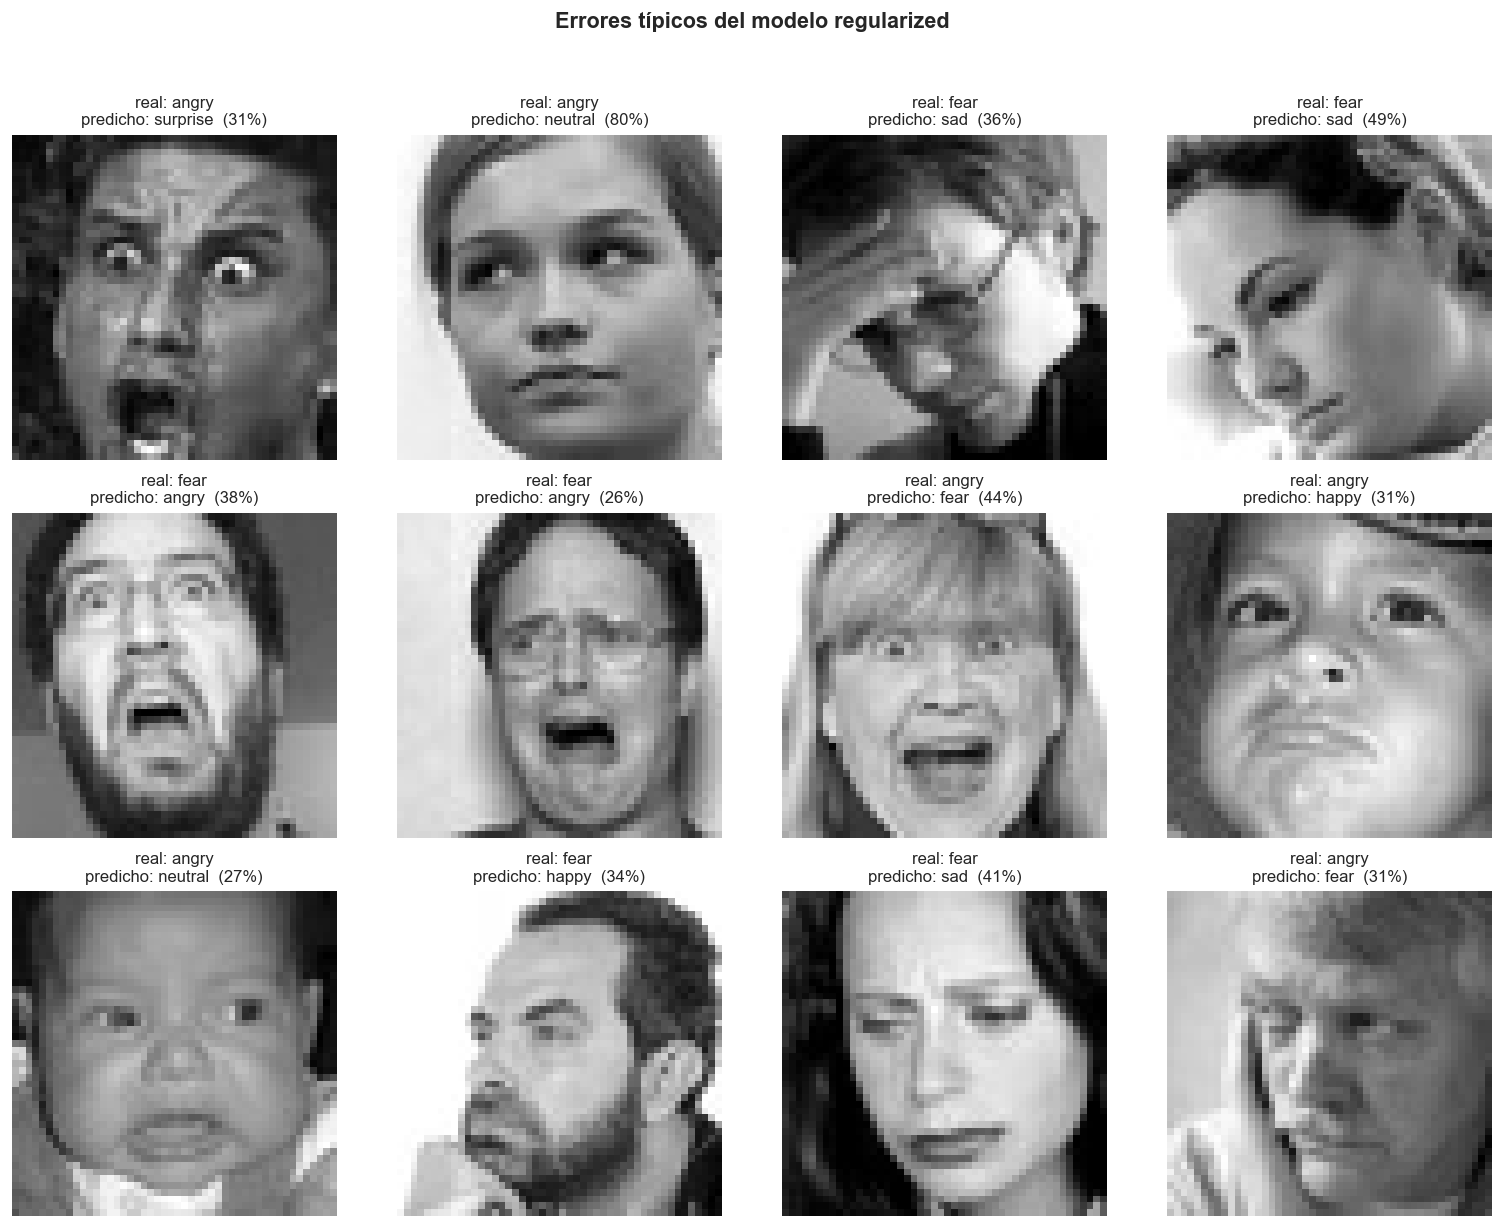
\includegraphics[width=\columnwidth]{../outputs/07_errores_cualitativos.png}
\caption{Errores típicos de la variante B (la ganadora por F1-macro). Una porción no trivial de los errores es \textit{interpretable}: \texttt{fear} confundido con \texttt{surprise} (ambas con ojos muy abiertos), \texttt{sad} confundido con \texttt{neutral} (ambas con boca cerrada y cejas relajadas). Esto es consistente con el techo informacional del dataset (accuracy humana sobre FER-2013 $\approx$65\,\%) y no necesariamente con una arquitectura insuficiente.}
\label{fig:errores}
\end{figure}

% =========================================================
%  6. DISCUSIÓN Y CONCLUSIONES
% =========================================================
\section{Discusión y conclusiones}

El experimento aporta dos hallazgos empíricos que matizan la intuición inicial. Primero, la regularización \textit{bien calibrada} (variante B) mejora claramente al baseline (+7,4 puntos de F1-macro), lo cual confirma su valor cuando la arquitectura tiene capacidad suficiente. Segundo, las defensas contra overfitting \textit{no son aditivas}: añadir aumentación sobre una red ya regularizada (variante C) produjo deterioro en lugar de mejora, en una arquitectura pequeña con $\sim$1,2 M de parámetros.

\paragraph{Resultado observado: A $<$ B $>$ C.} La progresión esperada A $\rightarrow$ B $\rightarrow$ C \textit{monotónicamente creciente} no se confirmó. En su lugar, observamos un máximo en B y un retroceso en C. Esto es coherente con dos hechos: (i) el modelo es lo bastante pequeño como para que una segunda capa de regularización lo lleve a underfitting (\textit{train\_acc} de C: 0,45 vs B: 0,60); (ii) la interacción de \texttt{BatchNormalization} con \texttt{restore\_best\_weights} introduce inconsistencia entre los pesos restaurados de la mejor época y las \textit{running statistics} acumuladas durante todo el entrenamiento.

Lejos de invalidar el experimento, este resultado lo refuerza: el feedback de la Semana 1 ya había documentado un patrón análogo (L2 con $\lambda=0,01$ \textit{empeoró} el baseline). La lección recurrente es que cada técnica de regularización requiere calibración en su escala propia y que las defensas se suman \textit{no linealmente} al combinarse en arquitecturas pequeñas. La estrategia metodológica de \textit{añadir una sola familia de cambios por iteración} --- el feedback explícito del docente --- es precisamente lo que permitió aislar este efecto y atribuirlo a la decisión de añadir aumentación, sin ambigüedad.

\subsection{Lecciones aprendidas y trabajo futuro}

\textbf{Conceptual:} la decisión de centralizar la arquitectura en una sola función \texttt{build\_cnn(...)} con \textit{flags} es lo que vuelve atribuible cada mejora. Sin esta restricción de diseño, una variante mejor no permitiría saber \textit{cuál} de las decisiones produjo el efecto. \textbf{Operativo:} en contextos psicoeducativos --- aplicación natural de este modelo --- el F1-macro es preferible a la accuracy precisamente porque trata las siete emociones como igualmente relevantes; ignorar \texttt{disgust} o \texttt{fear} sería problemático para una aplicación clínica asistida. \textbf{Ético:} este modelo clasifica patrones visuales en imágenes, no estados emocionales internos (Barrett et al., 2019). FER-2013 tiene además ruido de etiquetado documentado (accuracy humana $\approx$ 65\,\%). Cualquier uso aplicado requiere validación con poblaciones representativas y supervisión clínica.

\textbf{Limitaciones reconocidas y trabajo futuro:}
\begin{enumerate}[label=\roman*.]
    \item Probar arquitecturas más profundas (3 bloques convolucionales, filtros 32$\rightarrow$64$\rightarrow$128) para cuantificar el aporte real de la profundidad. Una red más grande probablemente absorbería la aumentación de C sin caer en underfitting.
    \item Investigar el comportamiento de \texttt{BatchNormalization} con \texttt{restore\_best\_weights}: re-entrenar la variante C \textit{sin} restauración para confirmar si el gap val--test de C se debe a inconsistencia de \textit{moving stats}.
    \item Implementar validación cruzada \textit{k-fold} con múltiples semillas para reducir varianza en las métricas reportadas (especialmente relevante dado el comportamiento atípico de C).
    \item Explorar estrategias alternativas de manejo del desbalance: \textit{oversampling} con SMOTE adaptado a imágenes, o muestreo balanceado por lote --- evitando el efecto desestabilizador que tuvo \texttt{class\_weight} en este experimento.
    \item \textbf{Semana 3 --- Transfer Learning:} cargar una red pre-entrenada (MobileNetV2 sobre ImageNet o VGG-Face sobre rostros), congelar las convolucionales y re-entrenar la cabeza para FER-2013. La hipótesis de cierre es que el transfer aportará una mejora $\geq$\,+5 puntos de F1-macro sobre la mejor variante de esta semana (B con F1=0,5032), gracias a representaciones visuales generales que una CNN entrenada desde cero sobre $\sim$29.000 imágenes no alcanza a aprender por sí sola.
\end{enumerate}

% =========================================================
%  CIERRE DEL FEEDBACK PROFESORAL
% =========================================================
\section{Cierre del feedback profesoral (40/40)}

\textit{Sección añadida en la entrega final del cuatrimestre para documentar cómo el feedback sobre esta práctica se aplicó en Semana 3.}

\paragraph{Comentario del docente.} \textit{``Felicitaciones la práctica ha estado muy bien desarrollada y explicada. (\ldots) Yo quitaría de la red las capas de MaxPooling basado en que la imagen es 48$\times$48$\times$1 (poca información); el objetivo principal del pooling es reducir computación pero aquí quizás esté quitando características importantes. (\ldots) Esta semana podrían expandir más la exploración con fine tuning y redes más grandes con regularización adecuada para ver el comportamiento.''}

\paragraph{Acciones aplicadas en Semana 3.} (i) El backbone elegido, \textbf{MobileNetV2}, \textit{no usa MaxPooling} por diseño — emplea \texttt{Conv2D(stride=2)} para el downsampling. Adicionalmente las imágenes se redimensionaron a 96$\times$96 RGB. (ii) Toda Semana 3 es una respuesta directa a la segunda sugerencia: backbone de 88 capas (3$\times$ la profundidad de la CNN actual) entrenado en dos fases con LR diferenciado 1\,000$\times$ (\texttt{1e-3} en Feature Extraction y \texttt{1e-5} en Fine-Tuning). El delta interno entre fases fue $+3{,}07$\,pp F1, validando empíricamente la estrategia. (iii) Sobre el desbalance: en Semana 3 se evitó deliberadamente reintroducir \texttt{class\_weight} tras el hallazgo de esta práctica.

\paragraph{Hallazgo cruzado con Semana 3.} Sorprendentemente, el Transfer Learning con MobileNetV2/ImageNet \textbf{no superó} a la mejor variante de esta semana (F1\,=\,0,3814 vs 0,5032). El análisis interno mostró que el fine-tuning sí añadió valor pero el techo del backbone es bajo por mismatch de dominio (ImageNet objetos naturales vs FER-2013 rostros 48$\times$48 grayscale). La intuición del docente sobre el MaxPooling se confirmó válida, pero el cuello de botella efectivo está en otro lado (backbone genérico). Esto refuerza el patrón observado en Semana 1: las técnicas sofisticadas requieren calibración al problema, no se asumen.

% =========================================================
%  Referencias breves (estilo del informe Semana 1: en línea)
% =========================================================
\paragraph{Referencias.}
{\footnotesize
Goodfellow, I. et al. (2013). \textit{Challenges in Representation Learning}, ICML Workshop. ~$\bullet$~
Ioffe, S. \& Szegedy, C. (2015). \textit{Batch Normalization}, arXiv:1502.03167. ~$\bullet$~
Srivastava, N. et al. (2014). \textit{Dropout}, JMLR 15:1929--1958. ~$\bullet$~
Barrett, L. F. et al. (2019). \textit{Emotional Expressions Reconsidered}, Psychological Science in the Public Interest 20(1):1--68.
}

\end{document}
